% Copyright 2019 Clara Eleonore Pavillet

% Author: Clara Eleonore Pavillet
% Description: This is an unofficial Oxford University Beamer Template I made from scratch. Feel free to use it, modify it, share it.
% Version: 1.0

\documentclass{beamer}
\usepackage{pdfpages}
% Load Packages
\usepackage[utf8]{inputenc}
\usepackage{xcolor}
\usepackage{tikz}
\usetikzlibrary{positioning,calc}
\usepackage{graphicx}
\usepackage{hyperref}
\usepackage{amsmath}
\usepackage{listings}
\usepackage{fontawesome}
\usepackage[T2A]{fontenc}
\usepackage[utf8]{inputenc}
\usepackage[russian]{babel}

% Define Commands
\newcommand*{\ClipSep}{0.06cm} %To adjust footer logo
\newcommand{\E}{\mathrm{e}\,} %\def\I{e} % used to defined e for exp(x), see later what it should be
\newcommand{\ud}{\mathrm{d}}
\lstset{numbers=left, numberstyle=\tiny, stepnumber=1,firstnumber=1,breaklines=true,
    numbersep=5pt,language=Python,
    stringstyle=\ttfamily,
    basicstyle=\footnotesize, 
    showstringspaces=false
}

\usetheme{oxonian}
\usepackage{wrapfig}
\usepackage{listings}

\title{Използване на OpenMP.}
\subtitle{\textit{Курс „Паралелно програмиране“}}
\titlegraphic{{
\includegraphics[width=5.3cm]{iaps.png}}} 

\author{\newline \newline Стоян Мишев}

\vspace{1cm}

\date{} %\today

\begin{document}
\lstset{language=Python}
{\setbeamertemplate{footline}{} 
\frame{\titlepage}}


\section*{План}\begin{frame}{План}\tableofcontents\end{frame}

%%%%%%%%%%%%%%%%%%%%%%%%%%%%%%%%%%%%%

\begin{frame}[plain]{Задача}

  \begin{equation}
    \int_0^1 \frac{4}{1+x^2} dx = \pi  \nonumber
  \end{equation} \pause
\centering
  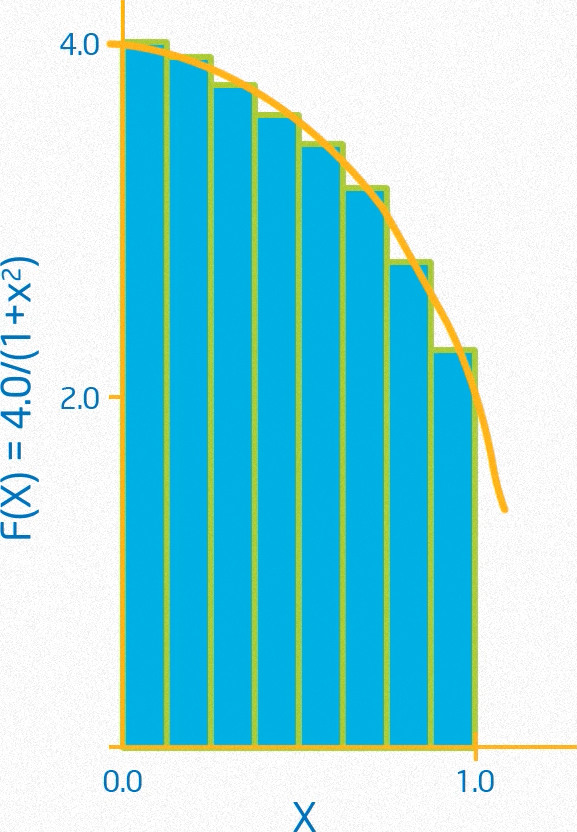
\includegraphics[width=0.5\textwidth]{integral-graph}

\end{frame}

\begin{frame}[fragile, plain]
  \frametitle{Решение без паралелни изчисления}
  \scriptsize
\lstset{language=C++}
    \begin{lstlisting}
#include <stdio.h>
#include <omp.h>
static long num_steps = 100000000;
double step;
int main ()
{
	  int i;
	  double x, pi, sum = 0.0;
	  double start_time, run_time;
	  step = 1.0/(double) num_steps;
	  start_time = omp_get_wtime();
	  for (i=1;i<= num_steps; i++){
		  x = (i-0.5)*step;
		  sum = sum + 4.0/(1.0+x*x);
	  }

	  pi = step * sum;
	  run_time = omp_get_wtime() - start_time;
	  printf("\n pi with %ld steps is %lf in %lf seconds\n ",num_steps,pi,run_time);
}	  
    \end{lstlisting}
\end{frame}

\begin{frame}[fragile, plain]
  \frametitle{Решение с паралелни изчисления 1}
\scriptsize
\lstset{language=C++}
\begin{lstlisting}
#define MAX_THREADS 4
static long num_steps = 100000000;
double step;
int main ()
{
	  int i,j;
	  double pi, full_sum = 0.0;
	  double start_time, run_time;
	  double sum[MAX_THREADS];
	  step = 1.0/(double) num_steps;
   for (j=1;j<=MAX_THREADS ;j++) {
      omp_set_num_threads(j);
      full_sum=0.0;
      start_time = omp_get_wtime();
      #pragma omp parallel
      {
        int i;
	  int id = omp_get_thread_num();
	  int numthreads = omp_get_num_threads();
	  double x;
	  sum[id] = 0.0;

        if (id == 0) 
             printf(" num_threads = %d",numthreads);

	  for (i=id;i< num_steps; i+=numthreads){
		  x = (i+0.5)*step;
		  sum[id] = sum[id] + 4.0/(1.0+x*x);
	  }
      }
	for(full_sum = 0.0, i=0;i<j;i++)
	    full_sum += sum[i];
      pi = step * full_sum;
      run_time = omp_get_wtime() - start_time;
      printf("\n pi is %f in %f seconds %d thrds \n",pi,run_time,j);
   }
}	  
    \end{lstlisting}
  
\end{frame}

\begin{frame}[fragile, plain]
  \frametitle{Решение с паралелни изчисления 1}
\scriptsize
\lstset{language=C++}
\begin{lstlisting}
        if (id == 0) 
             printf(" num_threads = %d",numthreads);

	  for (i=id;i< num_steps; i+=numthreads){
		  x = (i+0.5)*step;
		  sum[id] = sum[id] + 4.0/(1.0+x*x);
	  }
      }
	for(full_sum = 0.0, i=0;i<j;i++)
	    full_sum += sum[i];
      pi = step * full_sum;
      run_time = omp_get_wtime() - start_time;
      printf("\n pi is %f in %f seconds %d thrds \n",pi,run_time,j);
   }
}	  
    \end{lstlisting}  
\end{frame}

\begin{frame}[fragile, plain]
  \frametitle{Решение с паралелни изчисления 1. Мащабируемост.}
\centering

\includegraphics[width=0.35\textwidth]{scaling}\pause

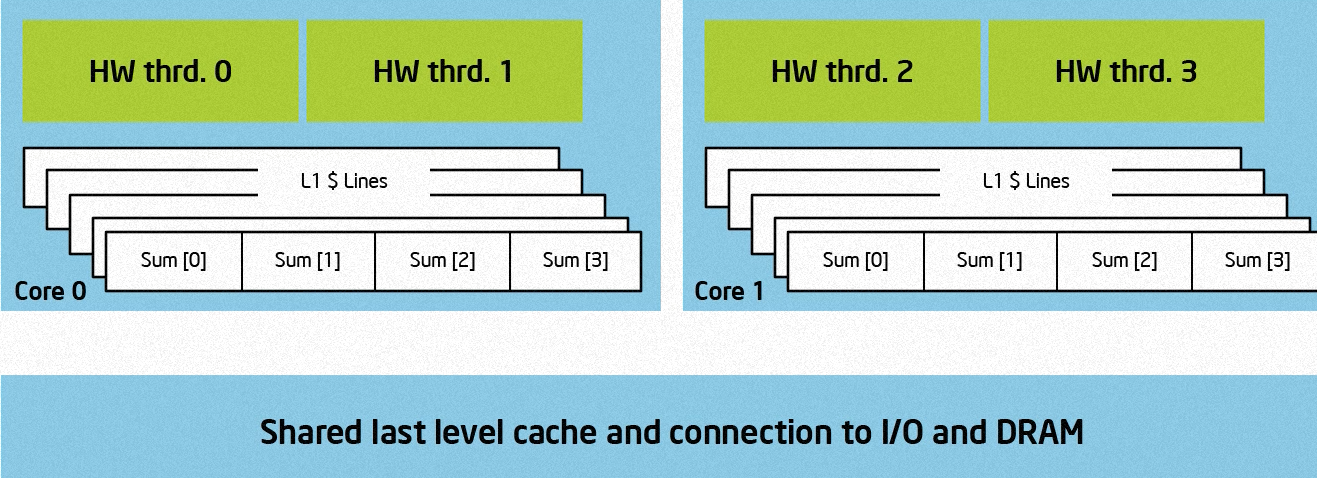
\includegraphics[width=\textwidth]{false-sharing}
\end{frame}

\begin{frame}[fragile, plain]
  \frametitle{Решение с паралелни изчисления 1. Отместване по L1.}
  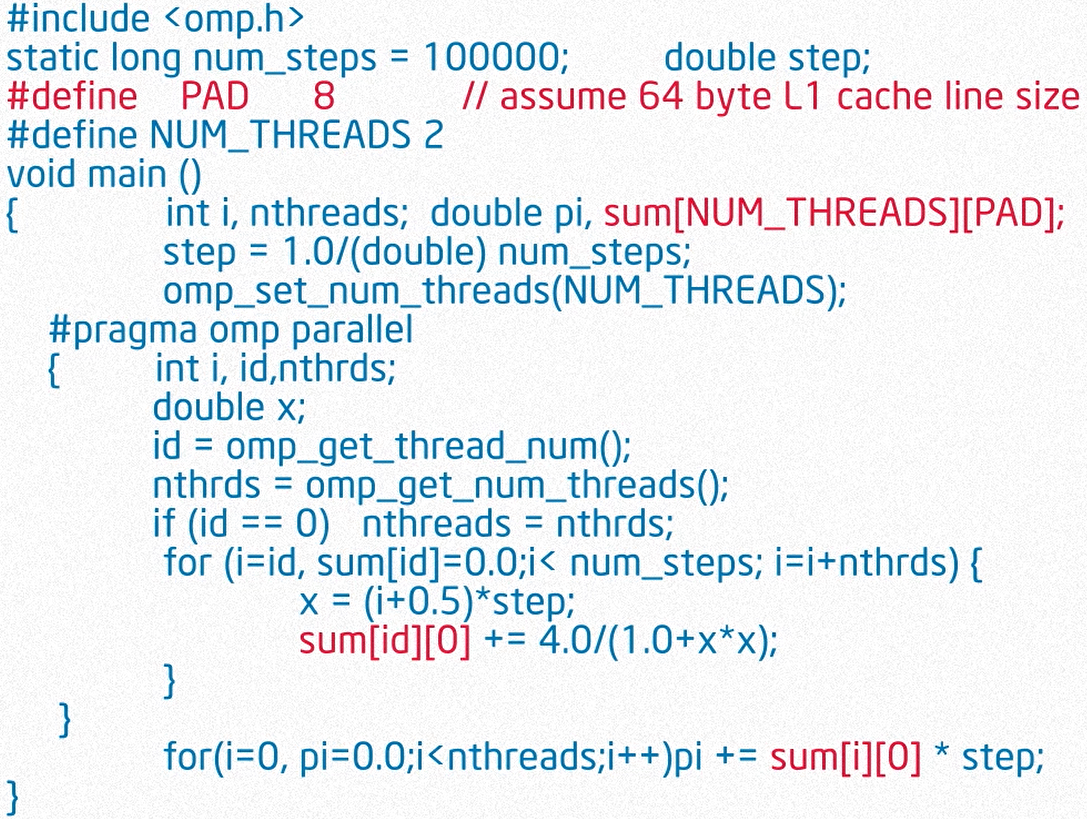
\includegraphics[width=\textwidth]{cache-line-overcome.png}
\end{frame}

\begin{frame}[fragile, plain]
  \frametitle{Решение с паралелни изчисления 2. Critical.}
  В част от програмата нишките се изпълняват последователно

  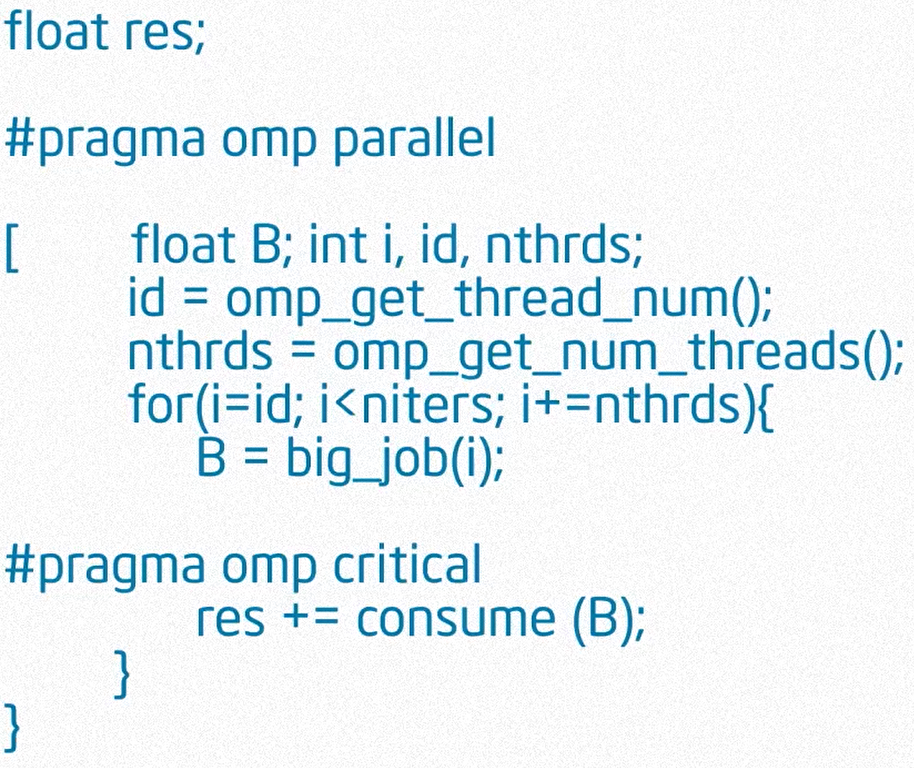
\includegraphics[width=0.8\textwidth]{critical}
\end{frame}

\begin{frame}[fragile, plain]
  \frametitle{Решение с паралелни изчисления 2. Critical.}
\scriptsize
\lstset{language=C++}
\begin{lstlisting}
#include <stdio.h>
#include <omp.h>

#define MAX_THREADS 4

static long num_steps = 100000000;
double step;
int main ()
{
	  int i,j;
	  double pi, full_sum = 0.0;
	  double start_time, run_time;
	  double sum[MAX_THREADS];

	  step = 1.0/(double) num_steps;


for(j=1;j<=MAX_THREADS ;j++){
   omp_set_num_threads(j);
   full_sum = 0.0;
	  start_time = omp_get_wtime();
\end{lstlisting}  
\end{frame}

\begin{frame}[fragile, plain]
  \frametitle{Решение с паралелни изчисления 2. Critical.}
\scriptsize
\lstset{language=C++}
\begin{lstlisting}
#pragma omp parallel private(i)
{
	  int id = omp_get_thread_num();
	  int numthreads = omp_get_num_threads();
	  double x;

	  double partial_sum = 0;

#pragma omp single
	  printf(" num_threads = %d",numthreads);

	  for (i=id;i< num_steps; i+=numthreads){
		  x = (i+0.5)*step;
		  partial_sum += + 4.0/(1.0+x*x);
	  }
#pragma omp critical
		  full_sum += partial_sum;
}
      
	  pi = step * full_sum;
	  run_time = omp_get_wtime() - start_time;
	  printf("\n pi is %f in %f seconds %d threds \n ",pi,run_time,j);
}
}	  
\end{lstlisting}  
\end{frame}

\begin{frame}[fragile]
\begin{lstlisting}
void avg_round_robin() {
    int N = 600000000;
    double tavg = 0;

    double timer_start = omp_get_wtime();
    omp_set_num_threads(16);
    #pragma omp parallel
    {
        double avg;
        int id = omp_get_thread_num();
        int nthreads = omp_get_num_threads();

        for (int i = id; i < N; i+=nthreads) {
            avg += i;
        }
        #pragma omp atomic
        tavg += avg;
    }
    double timer_elapsed = omp_get_wtime() - timer_start;
    tavg = tavg / N;

    std::cout << tavg << " took " << timer_elapsed << std::endl;
    //     1 threads took 2.1
    //     4 threads took 0.7
    //    48 threads took 0.65
}
\end{lstlisting}
\end{frame}


\begin{frame}
  \frametitle{Домашна работа}
\url{https://www.youtube.com/watch?v=cMWGeJyrc9w&list=PLLbPZJxtMs4ZHSamRRYCtvowRS0qIwC-I}  


До ``Introduction to OpenMP: 09 part 1 Module 5''

\end{frame}



\end{document}

%%% Local Variables:
%%% mode: latex
%%% TeX-master: t
%%% End:
